% This file was generated with po4a. Translate the source file.
%
\pdfobjcompresslevel=1 \documentclass[notes=hide]{beamer}
\usetheme[titlepagelogo=img2/cover]{LDN}

\usepackage[utf8]{inputenc}
\usepackage[francais]{babel}
\usepackage[T1]{fontenc}
\usepackage{tabularx, verbatim, xcolor, textpos}
\usepackage{lmodern, alltt, graphicx, ragged2e}
\usepackage{marvosym, multicol, textcomp, eurosym}

\definecolor{darkgreen}{RGB}{0,99,0}
\newcommand{\good}{{\color{green}\Smiley}}
\newcommand{\bad}{{\color{red}\Frowny}}
\colorlet{titre}{white} \setbeamercolor{normal text}{fg=white,bg=white}

\date{\textbf{PSES 2015}}

\title{La Brique Internet}
\subtitle{\vspace{10pt}\emph{Internet Neutre \& Auto-Hébergement}}
\author{Neutrinet \\ Lorraine Data Network \\ YunoHost}
\begin{document}

\begin{frame}[t,plain]
\titlepage
  \begin{textblock}{}(9.5,-6)
    
\includegraphics[height=1.5cm]{img2/logo-ynh-black.pdf}
  \end{textblock}
  \begin{textblock}{}(8.5,-3)
    
\includegraphics[height=1.2cm]{img2/ffdn}
  \end{textblock}
  {\color{black}\textbf{PSES -- 2015}}
\end{frame}

\watermarkon \watermarkoff
\setbeamercolor{background canvas}{bg=black}

\begin{frame}[t,plain]
  \begin{center}
    \vspace{\fill}
      \color{white}{\fontsize{60}{60}\selectfont libre, neutre et décentralisé}
    \vspace{\fill}
  \end{center}
\end{frame}

\begin{frame}[t,plain]
  \begin{center}
    \vspace{\fill}
      \color{white}{\fontsize{40}{40}\selectfont Libre et neutre~?}
    \vspace{\fill}
  \end{center}
\end{frame}

\begin{frame}[t]
\frametitle{\textcolor{titre}{Sans la Brique}}
  \color{red!60} % 60% de rouge mélanger avec la couleur donné à "titre" (donc 40%))""}
  \begin{center}
    \includegraphics[width=0.9\textwidth]{img2/connexion1.png}
  \end{center}
\end{frame}

\begin{frame}[t]
\frametitle{\textcolor{titre}{Sans la Brique}}
  \begin{center}
    \includegraphics[width=0.9\textwidth]{img2/connexion2.png}
  \end{center}
\end{frame}

\begin{frame}[t]
\frametitle{\textcolor{titre}{Sans la Brique}}
  \begin{center}
    \includegraphics[width=0.9\textwidth]{img2/connexion3.png}
  \end{center}
\end{frame}

\begin{frame}[t]
\frametitle{\textcolor{titre}{Sans la Brique}}
  \begin{center}
    \includegraphics[width=0.9\textwidth]{img2/connexion4.png}
  \end{center}
\end{frame}

\begin{frame}[t]
\frametitle{\textcolor{titre}{Problèmes~?}}
  \begin{center}
    \includegraphics[width=0.9\textwidth]{img2/connexion5.png}
  \end{center}
\end{frame}

\begin{frame}
\frametitle{\textcolor{titre}{Problèmes}}
  \begin{itemize}
    \item Bridage (Free/Youtube)
      \pause
    \item Blocage de port (Orange port 25)
      \pause
    \item Adressage IP dynamique / IPv6 (Orange)
      \pause
    \item Censure (DNS menteurs)
      \pause
    \item Surveillance (Boîtes noires ?)
      \pause
    \item Utilisation des données personnelles
  \end{itemize}
\end{frame}

\begin{frame}[t]
  \frametitle{\textcolor{titre}{Promesse de ne pas respecter ma vie privée}}
\begin{center}
\vfill
\includegraphics[width=.75\textwidth]{img2/03g-cgu.png}
\vfill
\end{center}
\end{frame}

\begin{frame}[t]
\frametitle{\textcolor{titre}{Avec la Brique}}
  \color{red!60} % 60% de rouge mélanger avec la couleur donné à "titre" (donc 40%))""}
  \begin{center}
  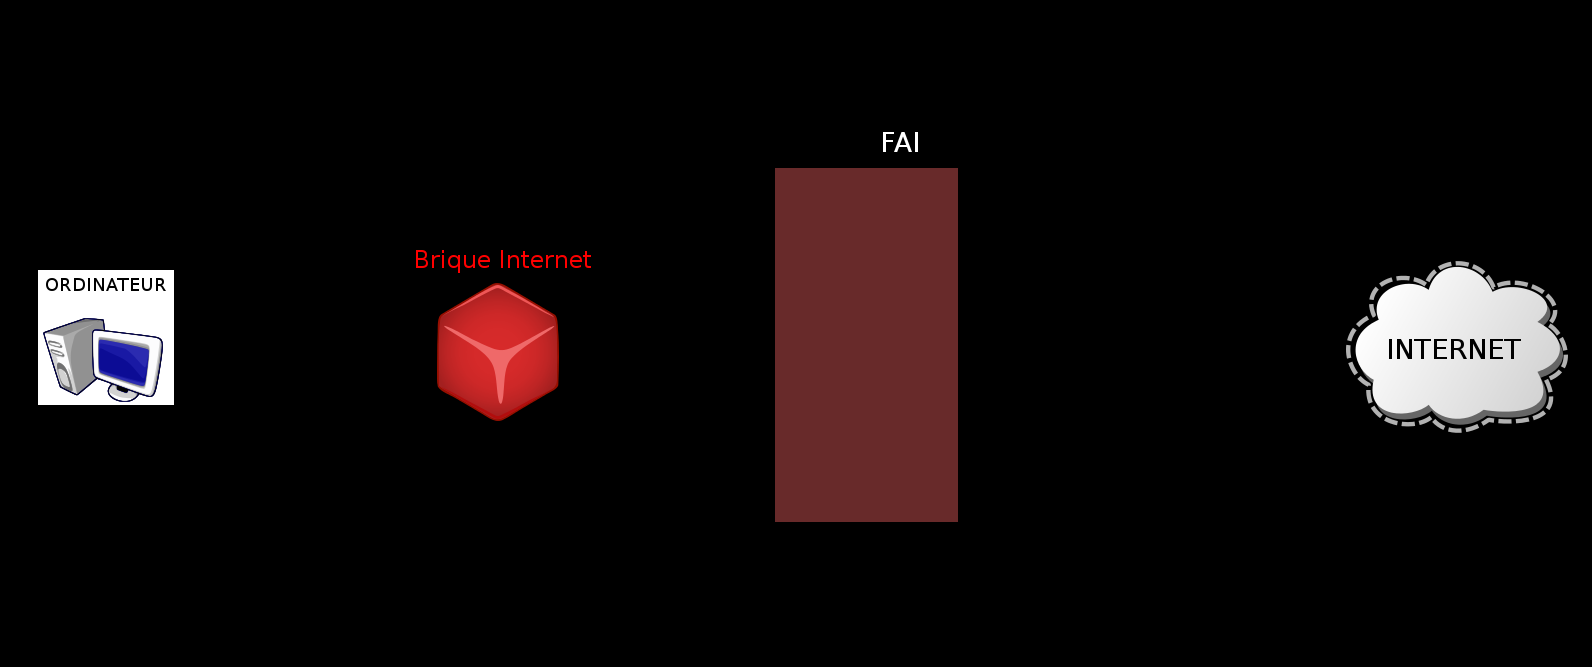
\includegraphics[width=0.9\textwidth]{img2/connexion11.png}
  \end{center}
\end{frame}
\begin{frame}[t]
\frametitle{\textcolor{titre}{Avec la Brique}}
  \begin{center}
  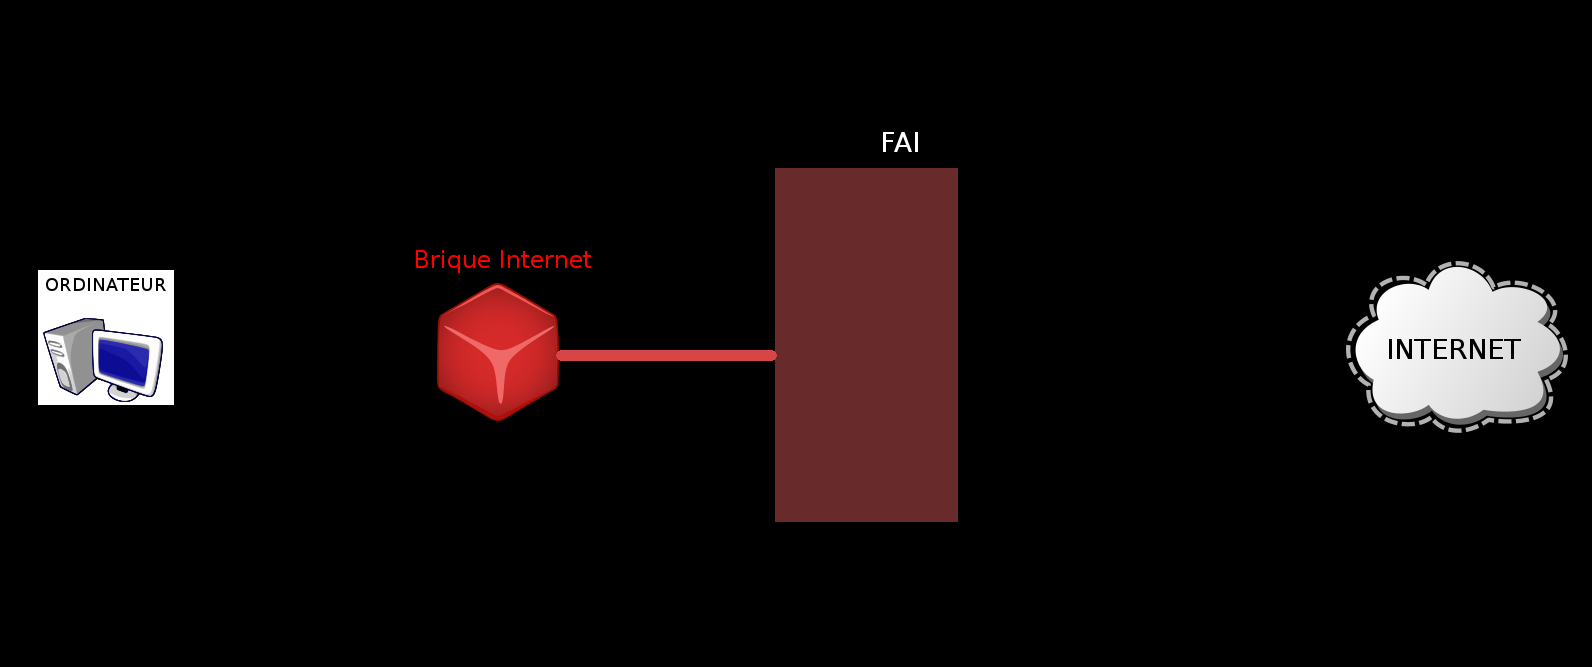
\includegraphics[width=0.9\textwidth]{img2/connexion12.png}
  \end{center}
\end{frame}
\begin{frame}[t]
\frametitle{\textcolor{titre}{Avec la Brique}}
  \begin{center}
  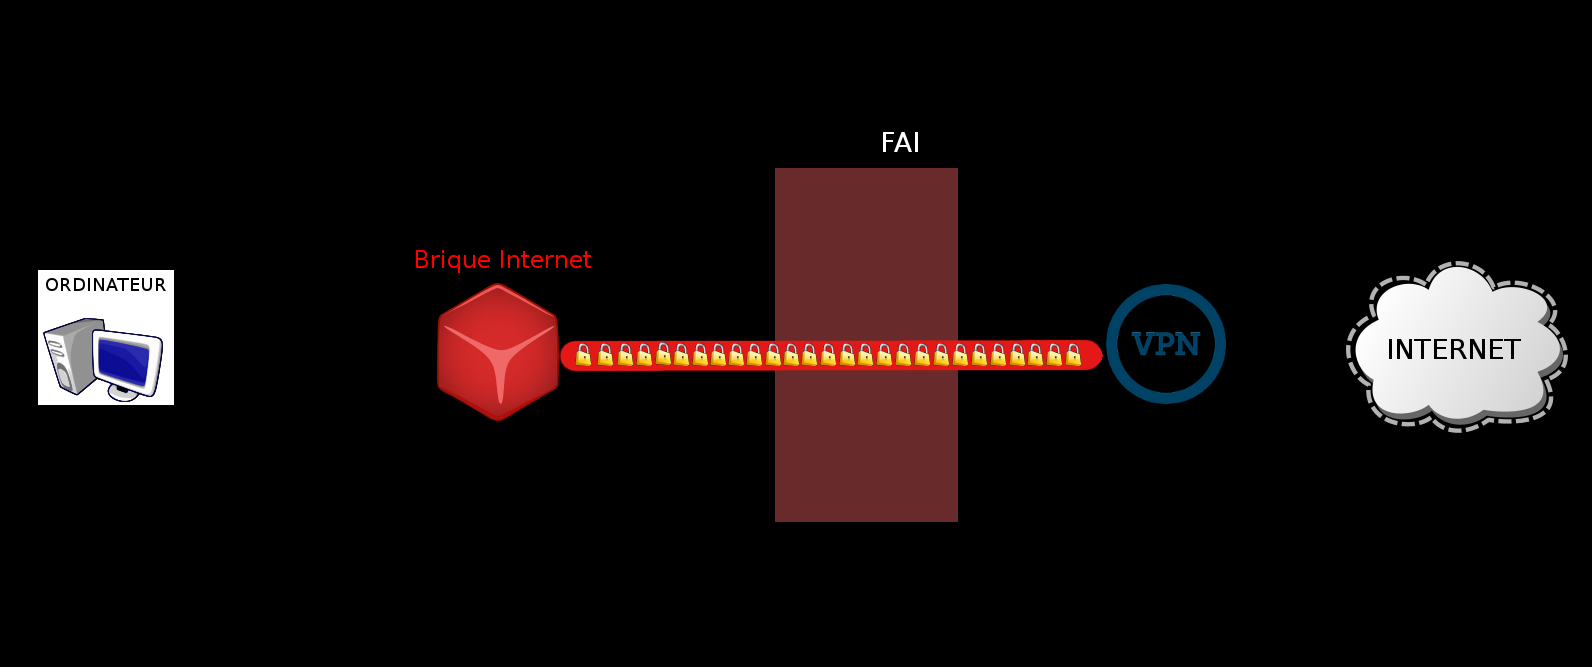
\includegraphics[width=0.9\textwidth]{img2/connexion13.png}
  \end{center}
\end{frame}
\begin{frame}[t]
\frametitle{\textcolor{titre}{Avec la Brique}}
  \begin{center}
  \includegraphics[width=0.9\textwidth]{img2/connexion14.png}
  \end{center}
\end{frame}

\begin{frame}[t]
  \frametitle{\textcolor{titre}{Avec la Brique}}
  \begin{center}
  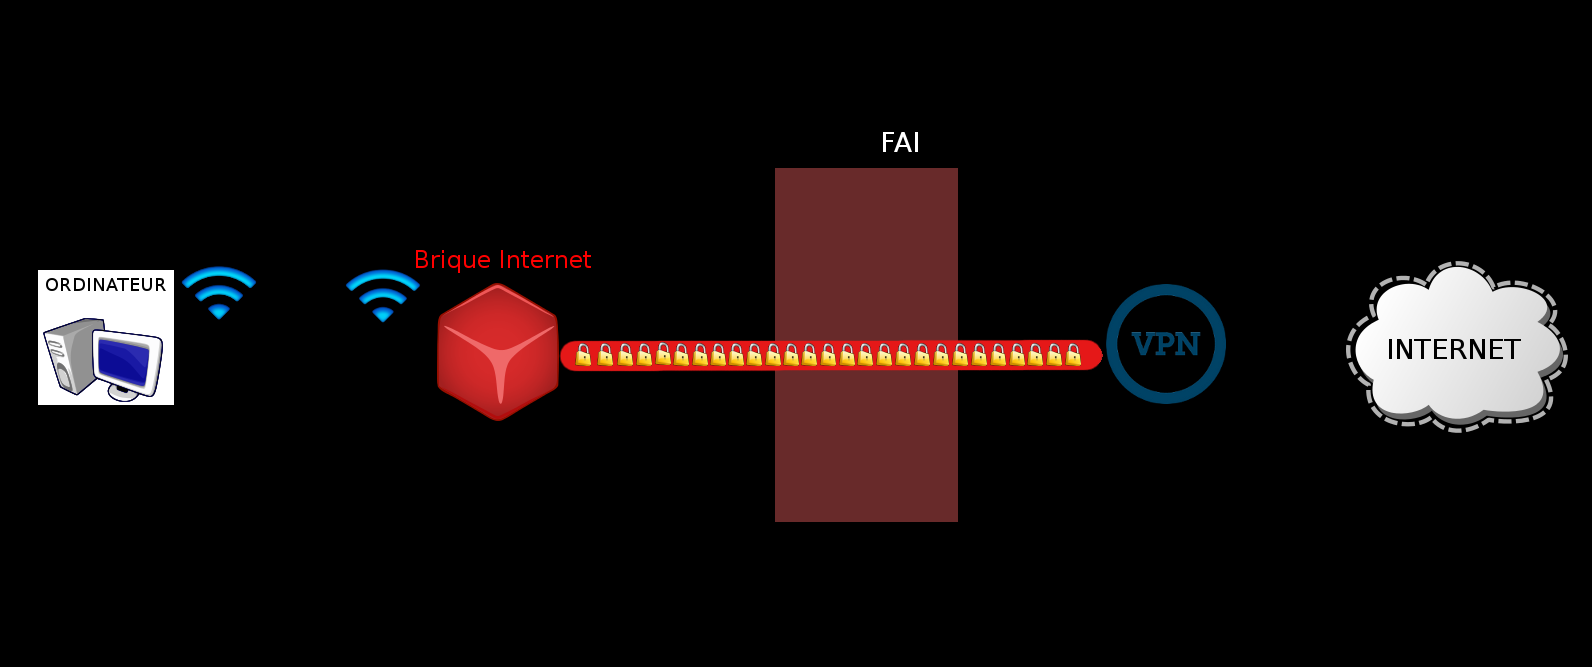
\includegraphics[width=0.9\textwidth]{img2/connexion15.png}
  \end{center}
\end{frame}

\begin{frame}[t]
  \frametitle{\textcolor{titre}{Avec la Brique}}
  \begin{center}
  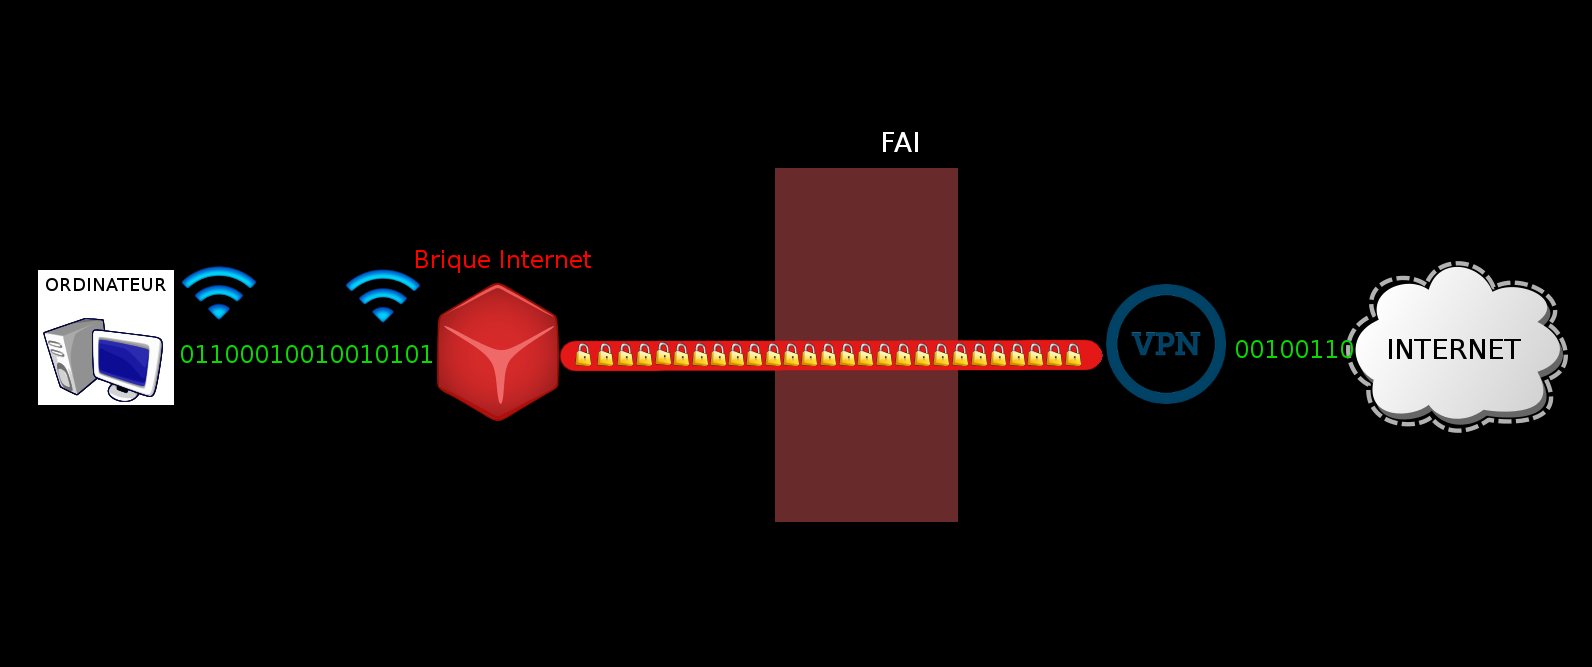
\includegraphics[width=0.9\textwidth]{img2/connexion16.png}
  \end{center}
\end{frame}

\begin{frame}
  \frametitle{\textcolor{titre}{Problèmes~?}}
  \begin{itemize}
    \item Bridage (YouTube/Free)
    \item Blocage de port (Orange port 25)
    \item Adressage IP dynamique / IPv6 (Orange)
    \item Censure (DNS menteurs)
    \item Surveillance (Boîtes noires ?)
    \item Utilisation des données personnelles
  \end{itemize}
\end{frame}

\begin{frame}
  \frametitle{\textcolor{titre}{Problèmes~?}}
  \begin{itemize}
    \item
    \item Blocage de port (Orange port 25)
    \item Adressage IP dynamique / IPv6 (Orange)
    \item Censure (DNS menteurs)
    \item Surveillance (Boîtes noires ?)
    \item Utilisation des données personnelles
  \end{itemize}
\end{frame}

\begin{frame}
  \frametitle{\textcolor{titre}{Problèmes~?}}
  \begin{itemize}
    \item
    \item
    \item Adressage IP dynamique / IPv6 (Orange)
    \item Censure (DNS menteurs)
    \item Surveillance (Boîtes noires ?)
    \item Utilisation des données personnelles
  \end{itemize}
\end{frame}

\begin{frame}
  \frametitle{\textcolor{titre}{Problèmes~?}}
  \begin{itemize}
    \item
    \item
    \item
    \item Censure (DNS menteurs)
    \item Surveillance (Boîtes noires ?)
    \item Utilisation des données personnelles
  \end{itemize}
\end{frame}

\begin{frame}
  \frametitle{\textcolor{titre}{Problèmes~?}}
  \begin{itemize}
    \item
    \item
    \item
    \item
    \item
    \item Utilisation des données personnelles
  \end{itemize}
\end{frame}

\begin{frame}
  \frametitle{\textcolor{titre}{Problèmes~?}}
  \begin{itemize}
    \item
    \item
    \item
    \item
    \item
    \item
  \end{itemize}
\end{frame}

\begin{frame}[t,plain]
\begin{center}
\vspace{\fill}
  \color{white}{\fontsize{60}{60}\selectfont libre, neutre!}
  \vspace{\fill}
\end{center}
\end{frame}

\begin{frame}[t,plain]
\begin{center}
\vspace{\fill}
  \color{white}{\fontsize{60}{60}\selectfont Décentralisé ?}
  \vspace{\fill}
\end{center}
\end{frame}
%sans la brique
%avec la brique
%solution
\begin{frame}[t]
  \frametitle{\textcolor{titre}{Comment communique-t-on sur Internet ?}}
\begin{center}
\vfill
\includegraphics[width=.7\textwidth]{img/15a-capture-gmailfbskype.png}
\vfill
\end{center}
\end{frame}

\begin{frame}[t]
  \frametitle{\textcolor{titre}{Ce que vous acceptez chez Google}}
  \vspace{4mm}
  \begin{justify}
« \emph{En soumettant des contenus à nos Services, par importation ou par tout autre moyen, \textbf{vous accordez à Google (et à toute personne travaillant avec Google) une licence}, dans le monde entier, d'utilisation, d'hébergement, de stockage, \textbf{de reproduction, de modification}, de création d’œuvres dérivées [...], de communication, de publication, de représentation publique, \textbf{d'affichage ou de distribution public desdits contenus.}} »\\
  \end{justify}
\end{frame}

\begin{frame}[t]
  \frametitle{\textcolor{titre}{Ce que vous acceptez chez Facebook}}
  \vspace{4mm}
  \begin{justify}
   « \emph{Pour le contenu protégé par les droits de propriété intellectuelle, comme les photos ou vidéos, [...] \textbf{vous nous accordez une licence} non-exclusive, \textbf{transférable, sous-licenciable}, sans redevance et mondiale \textbf{pour l'utilisation des contenus de propriété intellectuelle que vous publiez} sur Facebook ou en relation à Facebook} »
  \end{justify}
\end{frame}

\begin{frame}[t]
\frametitle{\textcolor{titre}{Pendant combien de temps chez Google~?}}
  \vspace{4mm}
  \begin{justify}
  « \emph{Cette autorisation demeure pour toute la durée légale de protection de votre contenu, \textbf{même si vous cessez d’utiliser nos Services}.} »
  \end{justify}
  \vspace{4mm}
\end{frame}

\begin{frame}[t]
\frametitle{\textcolor{titre}{Pendant combien de temps chez Facebook}}
  \vfill
\begin{justify}
   « \emph{Cette licence de propriété intellectuelle \textbf{se termine lorsque vous supprimez vos contenus} de propriété intellectuelle ou votre compte, \textbf{sauf si votre compte est partagé avec d'autres personnes} qui ne l'ont pas supprimé.} »\\
\end{justify}
\vfill
\begin{justify}
  « \emph{Lorsque vous supprimez votre contenu [...], vous comprenez que \textbf{les contenus supprimés peuvent persister dans des copies} de sauvegarde pendant \textbf{un certain temps}.} »
\end{justify}
\end{frame}

\begin{frame}[t]
\frametitle{\textcolor{titre}{Et avec la Brique Internet, cela se passe comment~?}}
\pause

\begin{center}

\includegraphics[width=\textwidth]{img2/yunohost_rien.png}
\end{center}
\end{frame}

\begin{frame}[t]
\begin{center}
\vfill
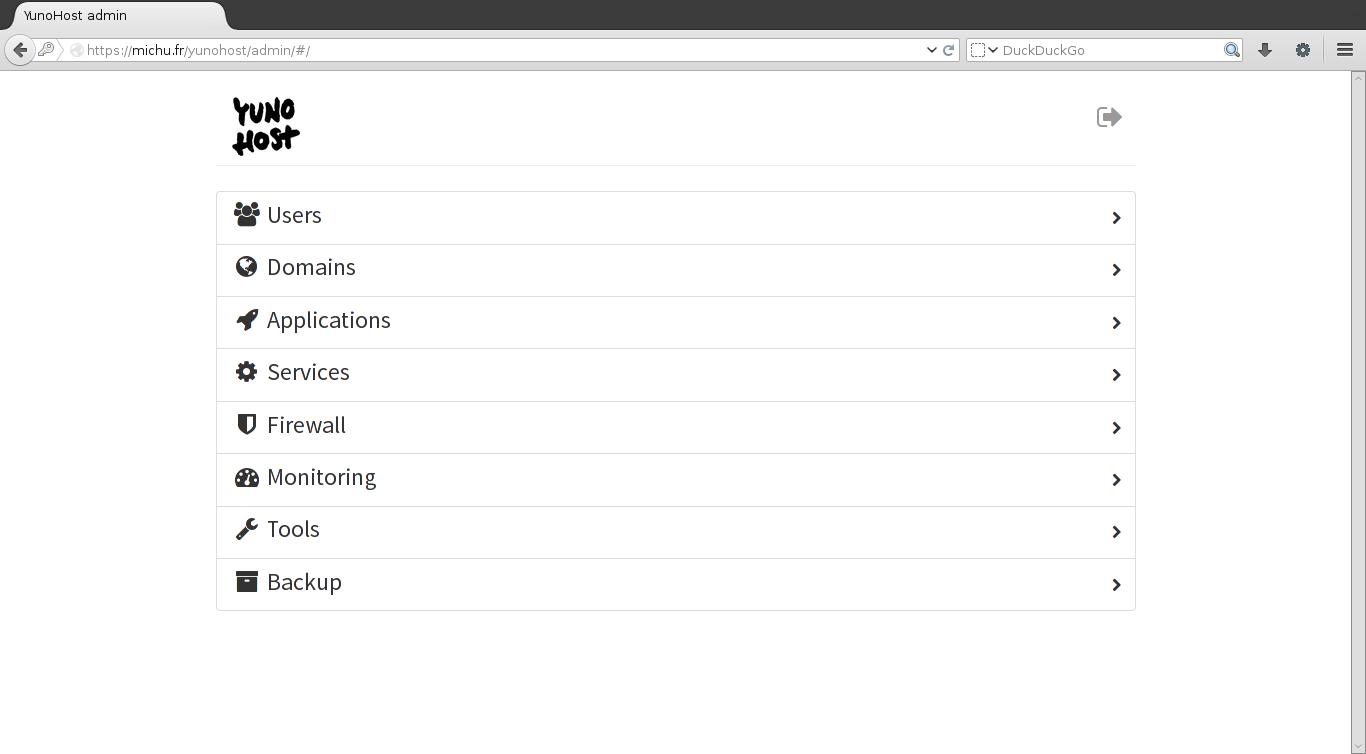
\includegraphics[width=\textwidth]{img2/17a-capture-yunohost.png}
\vfill
\end{center}
\end{frame}

\begin{frame}[t]
\begin{center}
\vfill
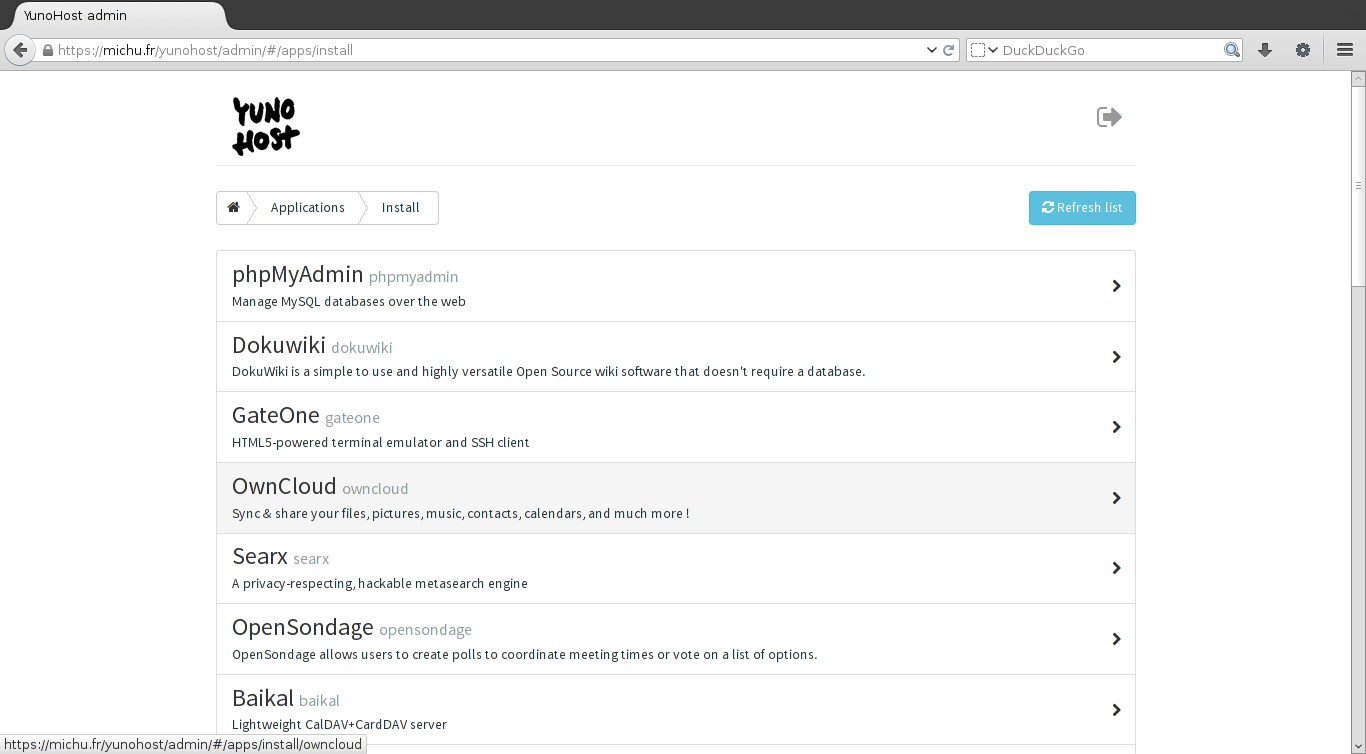
\includegraphics[width=\textwidth]{img2/19-capture-yunohostapps.png}
\vfill
\end{center}
\end{frame}

\begin{frame}[t,plain]
\begin{center}
\vspace{\fill}
  \color{white}{\fontsize{60}{60}\selectfont Décentralisé !}
  \vspace{\fill}
\end{center}
\end{frame}


\begin{frame}[t]
\frametitle{\textcolor{titre}{Combien ça coute…?}}
  \begin{center}
    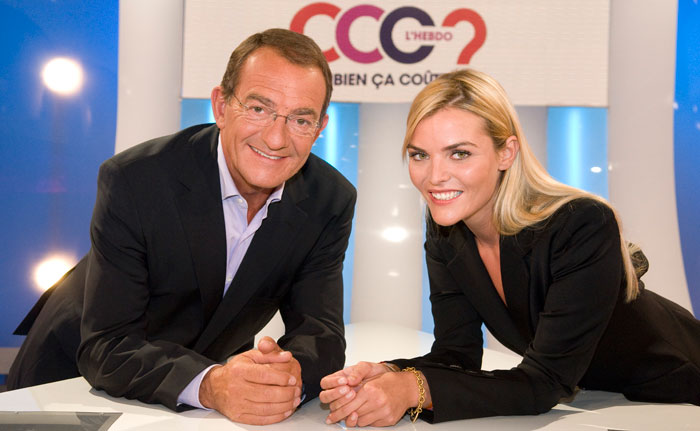
\includegraphics[width=0.9\textwidth]{img2/combiencacoute.jpg}
  \end{center}
\end{frame}

\begin{frame}[t]
\frametitle{\textcolor{titre}{Olimex}}
  \begin{center}
    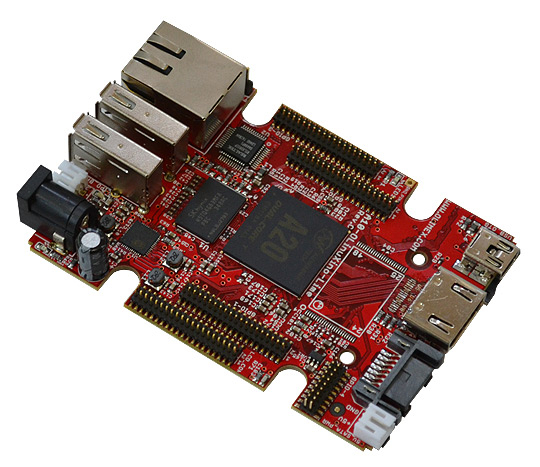
\includegraphics[width=0.7\textwidth]{img2/olimex.jpg}
  \end{center}
\end{frame}

\begin{frame}[t]
\frametitle{\textcolor{titre}{Boite}}
  \begin{center}
    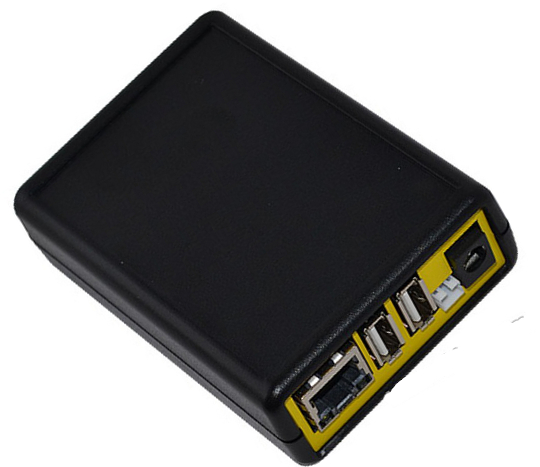
\includegraphics[width=0.7\textwidth]{img2/olimex-boite.jpg}
  \end{center}
\end{frame}
\begin{frame}[t]
\frametitle{\textcolor{titre}{Alimentation}}
  \begin{center}
    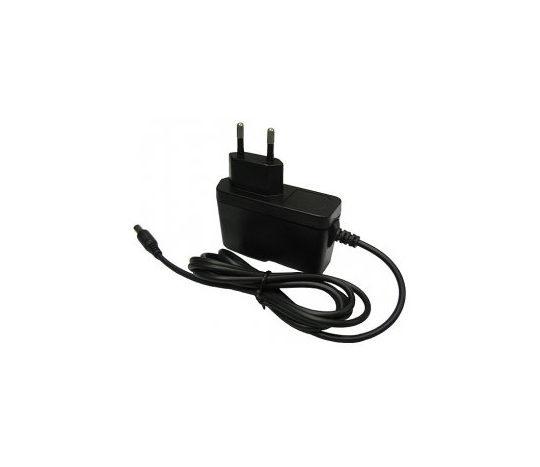
\includegraphics[width=0.7\textwidth]{img2/adaptateur.jpg}
  \end{center}
\end{frame}

\begin{frame}[t]
\frametitle{\textcolor{titre}{Antenne wifi}}
  \begin{center}
    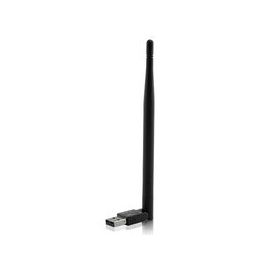
\includegraphics[width=0.6\textwidth]{img2/antenne.jpg}
  \end{center}
\end{frame}

\begin{frame}[t]
\frametitle{\textcolor{titre}{Carte mémoire}}
  \begin{center}
    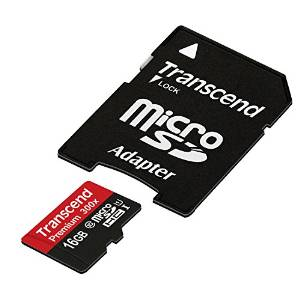
\includegraphics[width=0.6\textwidth]{img2/cartemem.jpg}
  \end{center}
\end{frame}

\begin{frame}[t]{}
\begin{center}
\vfill
\vfill
{\Large Environ \textbf{70\euro{} pour 1 Brique$^*$} complète \\ (frais de port inclus)}
\vspace{1cm}

{\Large Environ \textbf{7 \euro{} / mois} pour un \\ \textbf{accès VPN} associatif}
\vspace{1cm}
\vfill

{\footnotesize \emph{* pour une commande groupée > 9 Briques, sinon 80\euro}}
\vfill
\end{center}
\end{frame}

%\begin{frame}[t]
%\frametitle{\textcolor{titre}{J'ai une brique !}}
%\begin{center}
%  \vfill
%    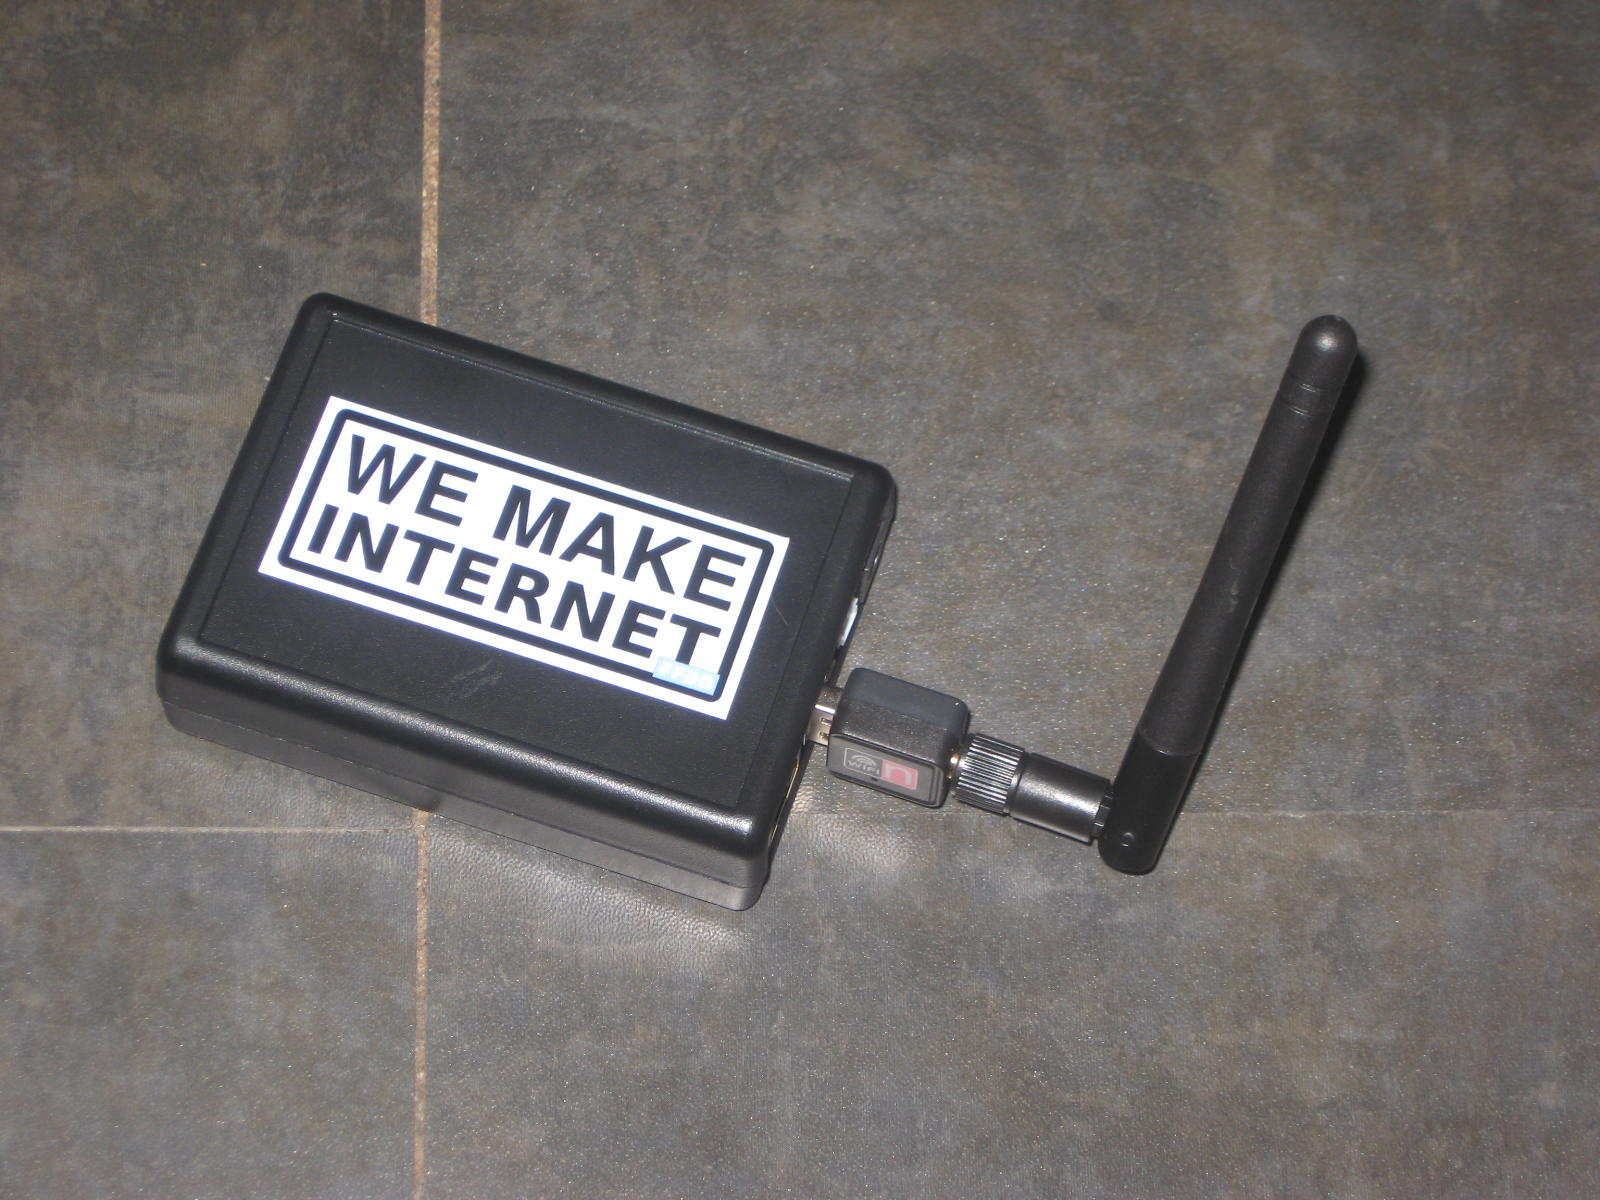
\includegraphics[width=.75\textwidth]{img2/04-photo-boitier.jpg}
%  \vfill
%\end{center}
%\end{frame}
%
%\begin{frame}[t]
%\frametitle{\textcolor{titre}{Je n'ai qu'a la brancher à ma box}}
%\begin{center}
%\vfill
%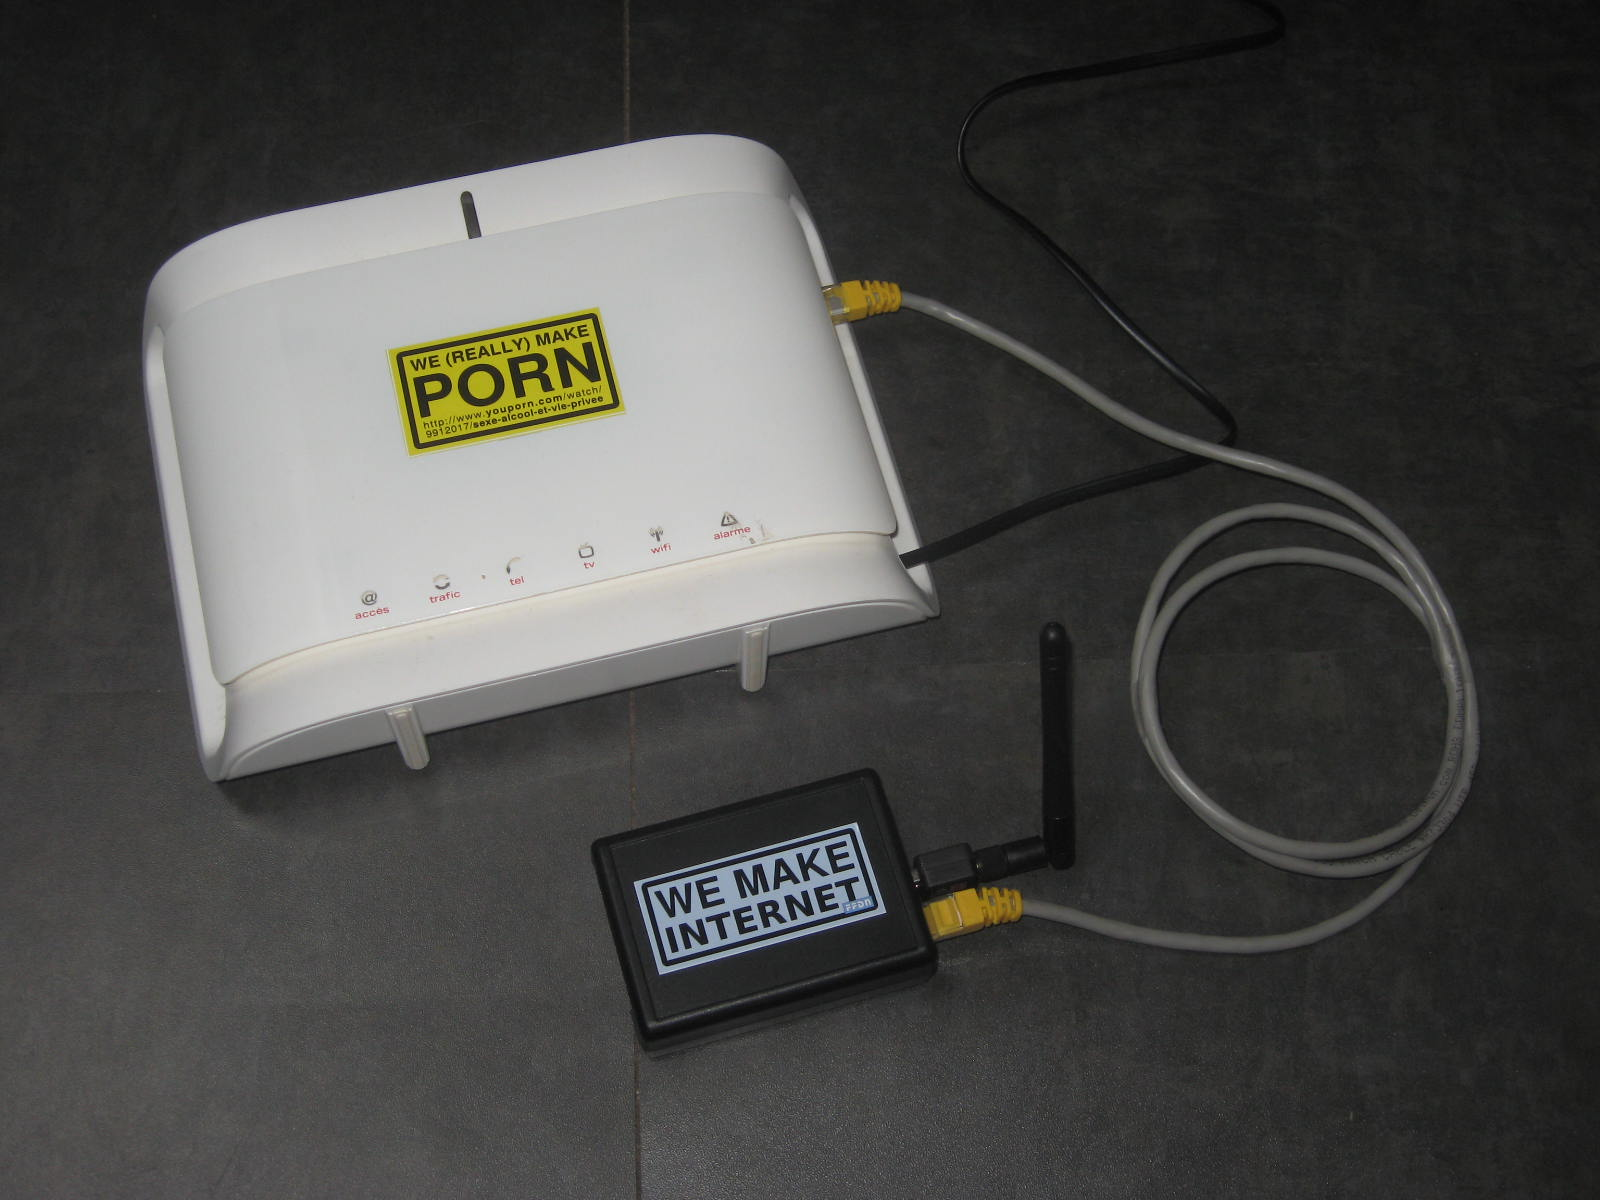
\includegraphics[width=.75\textwidth]{img2/05-photo-neufboxboitier.jpg}
%\vfill
%\end{center}
%\end{frame}
%
%\begin{frame}[t]
%\frametitle{\textcolor{titre}{Qui ne prend pas de place}}
%\begin{center}
%\vfill
%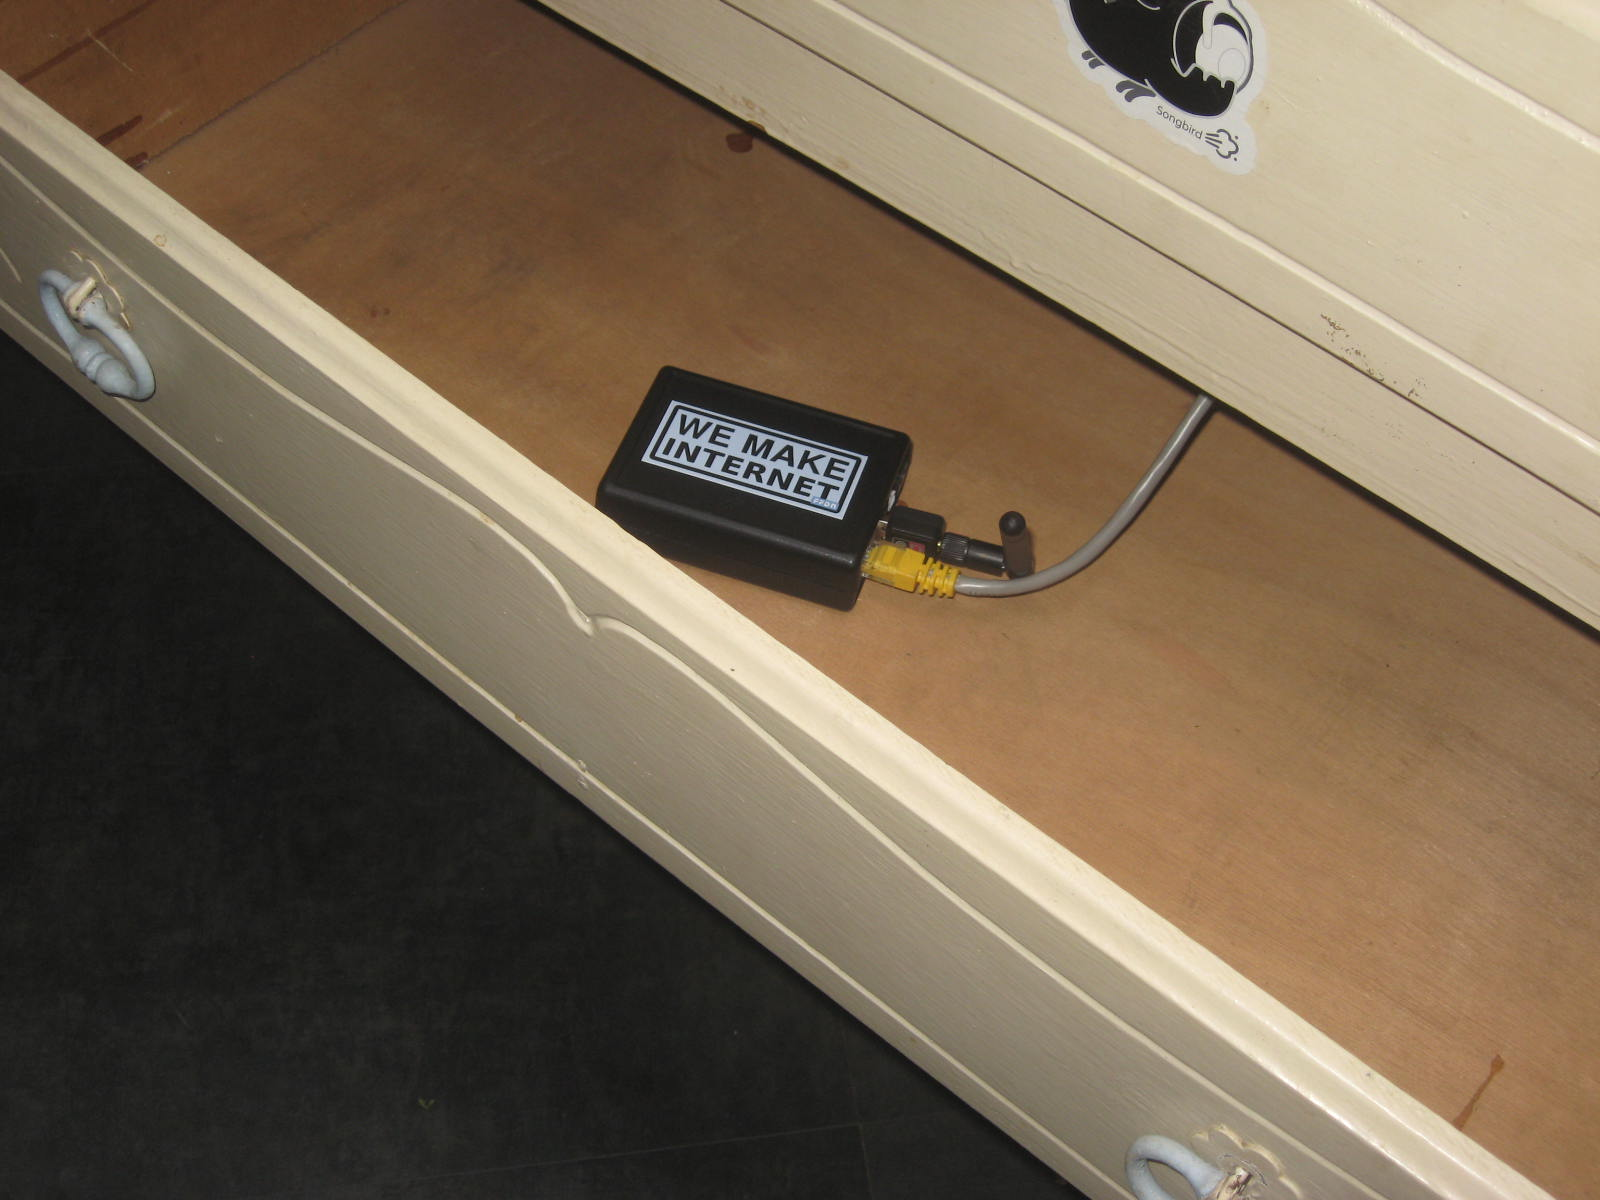
\includegraphics[width=.75\textwidth]{img2/16-photo-boitiercommode.jpg}
%\vfill
%\end{center}
%\end{frame}
%
%\begin{frame}[t]
%\frametitle{\textcolor{titre}{Et ça marche tout de suite}}
%\begin{center}
%\vfill
%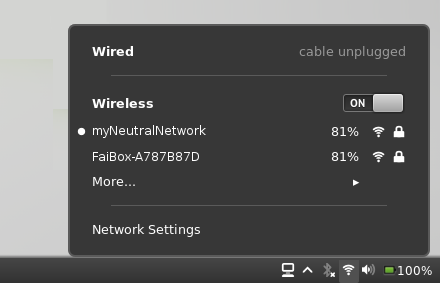
\includegraphics[width=.8\textwidth]{img2/06-capture-wifiboitier.png}
%\vfill
%\end{center}
%\end{frame}
%
%\begin{frame}[t]
%\frametitle{\textcolor{titre}{Je peux toujours utiliser les autres services de mon FAI}}
%\begin{center}
%\vfill
%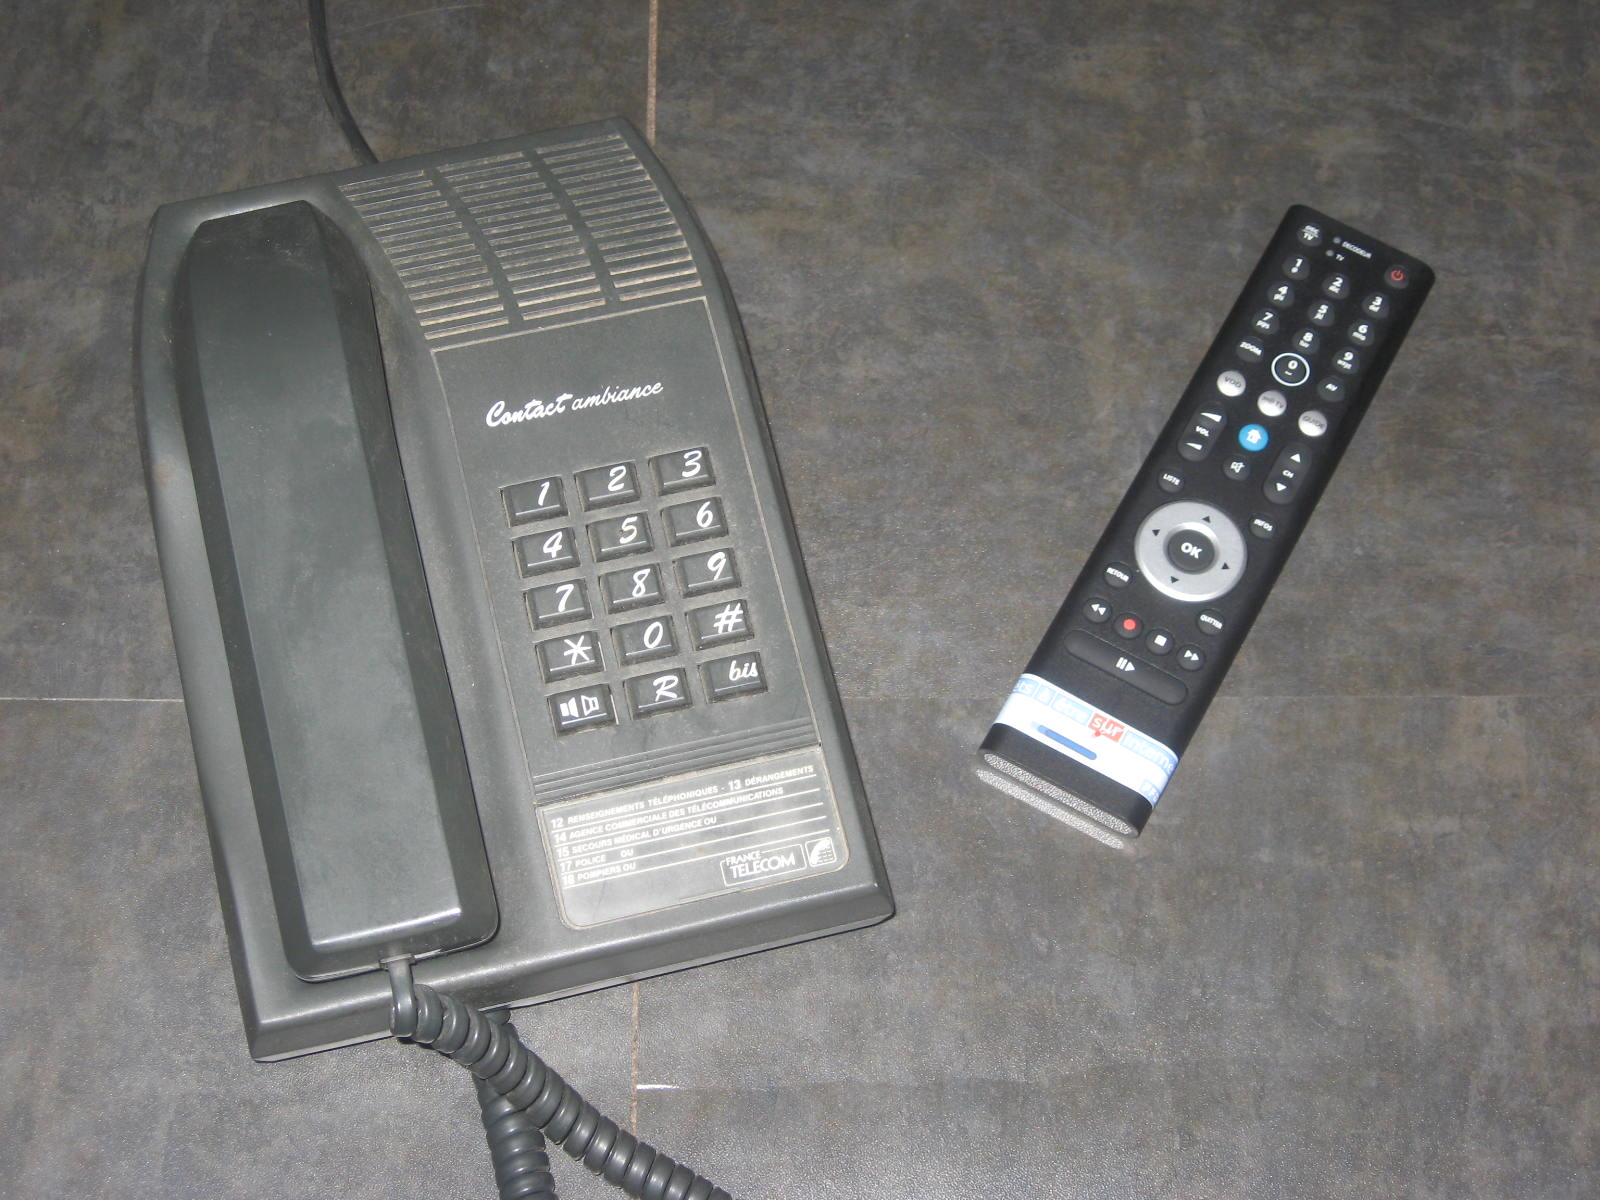
\includegraphics[width=.75\textwidth]{img2/13-photo-teltv.jpg}
%\vfill
%\end{center}
%\end{frame}

\begin{frame}[t]
\frametitle{\textcolor{titre}{La Brique Internet ?}}
\begin{center}
\vfill

\includegraphics[width=.6\textwidth]{img2/Shut-up-and-take-my-money.jpg}
\vfill
\end{center}
\end{frame}



%ou obtenir une brique ?
\begin{frame}[t]{}
\begin{center}
\vfill
{\Huge \textbf{Où trouver ce boîtier ?}}
\vspace{.5cm}

{\large \emph{Parce qu'il n'y en a pas à Carrefour, ni chez Amazon (pas encore)}}
\vfill
\end{center}
\end{frame}

\begin{frame}[t]
\frametitle{\textcolor{titre}{Dans des associations locales}}
\begin{center}
\vfill
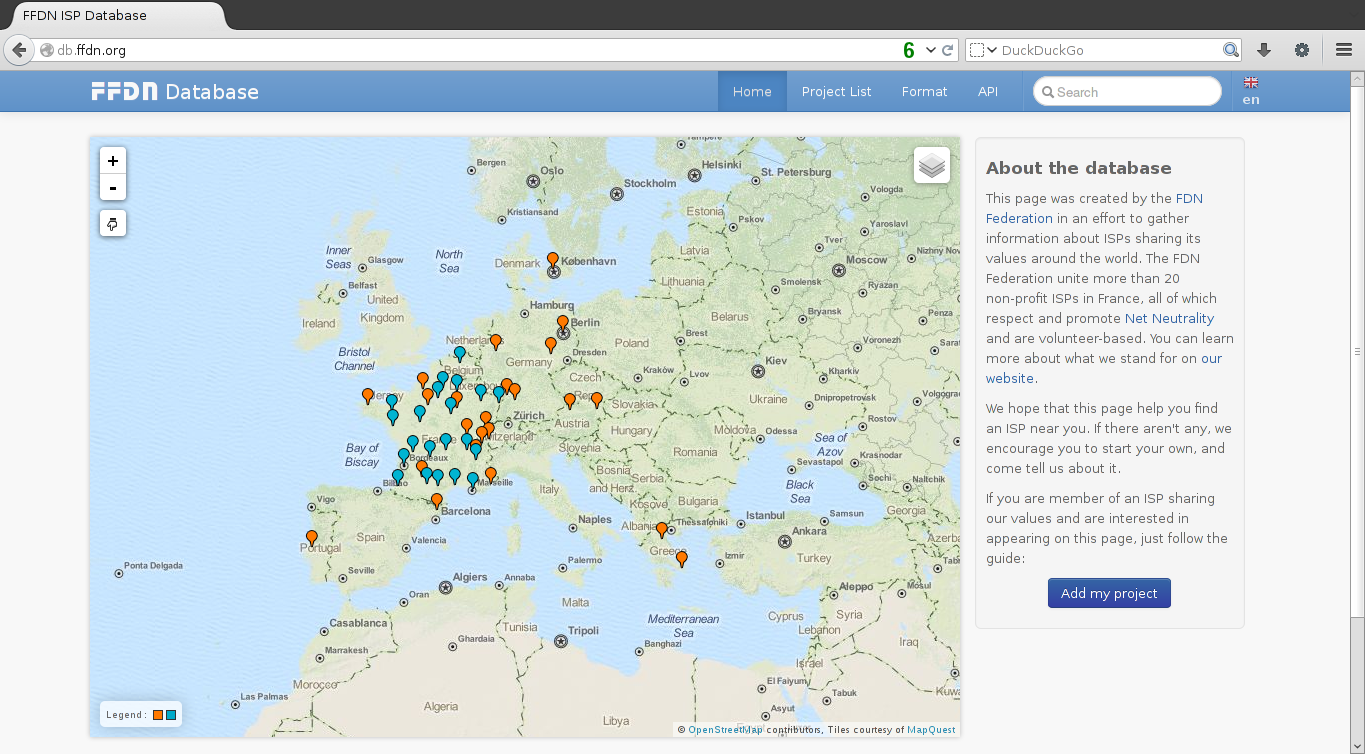
\includegraphics[width=\textwidth]{img2/25a-capture-ffdn.png}
\vfill
\end{center}
\end{frame}

\begin{frame}[t]
\frametitle{\textcolor{titre}{Ou le faire soi-même, puisque tout est libre}}
\begin{center}
\vfill
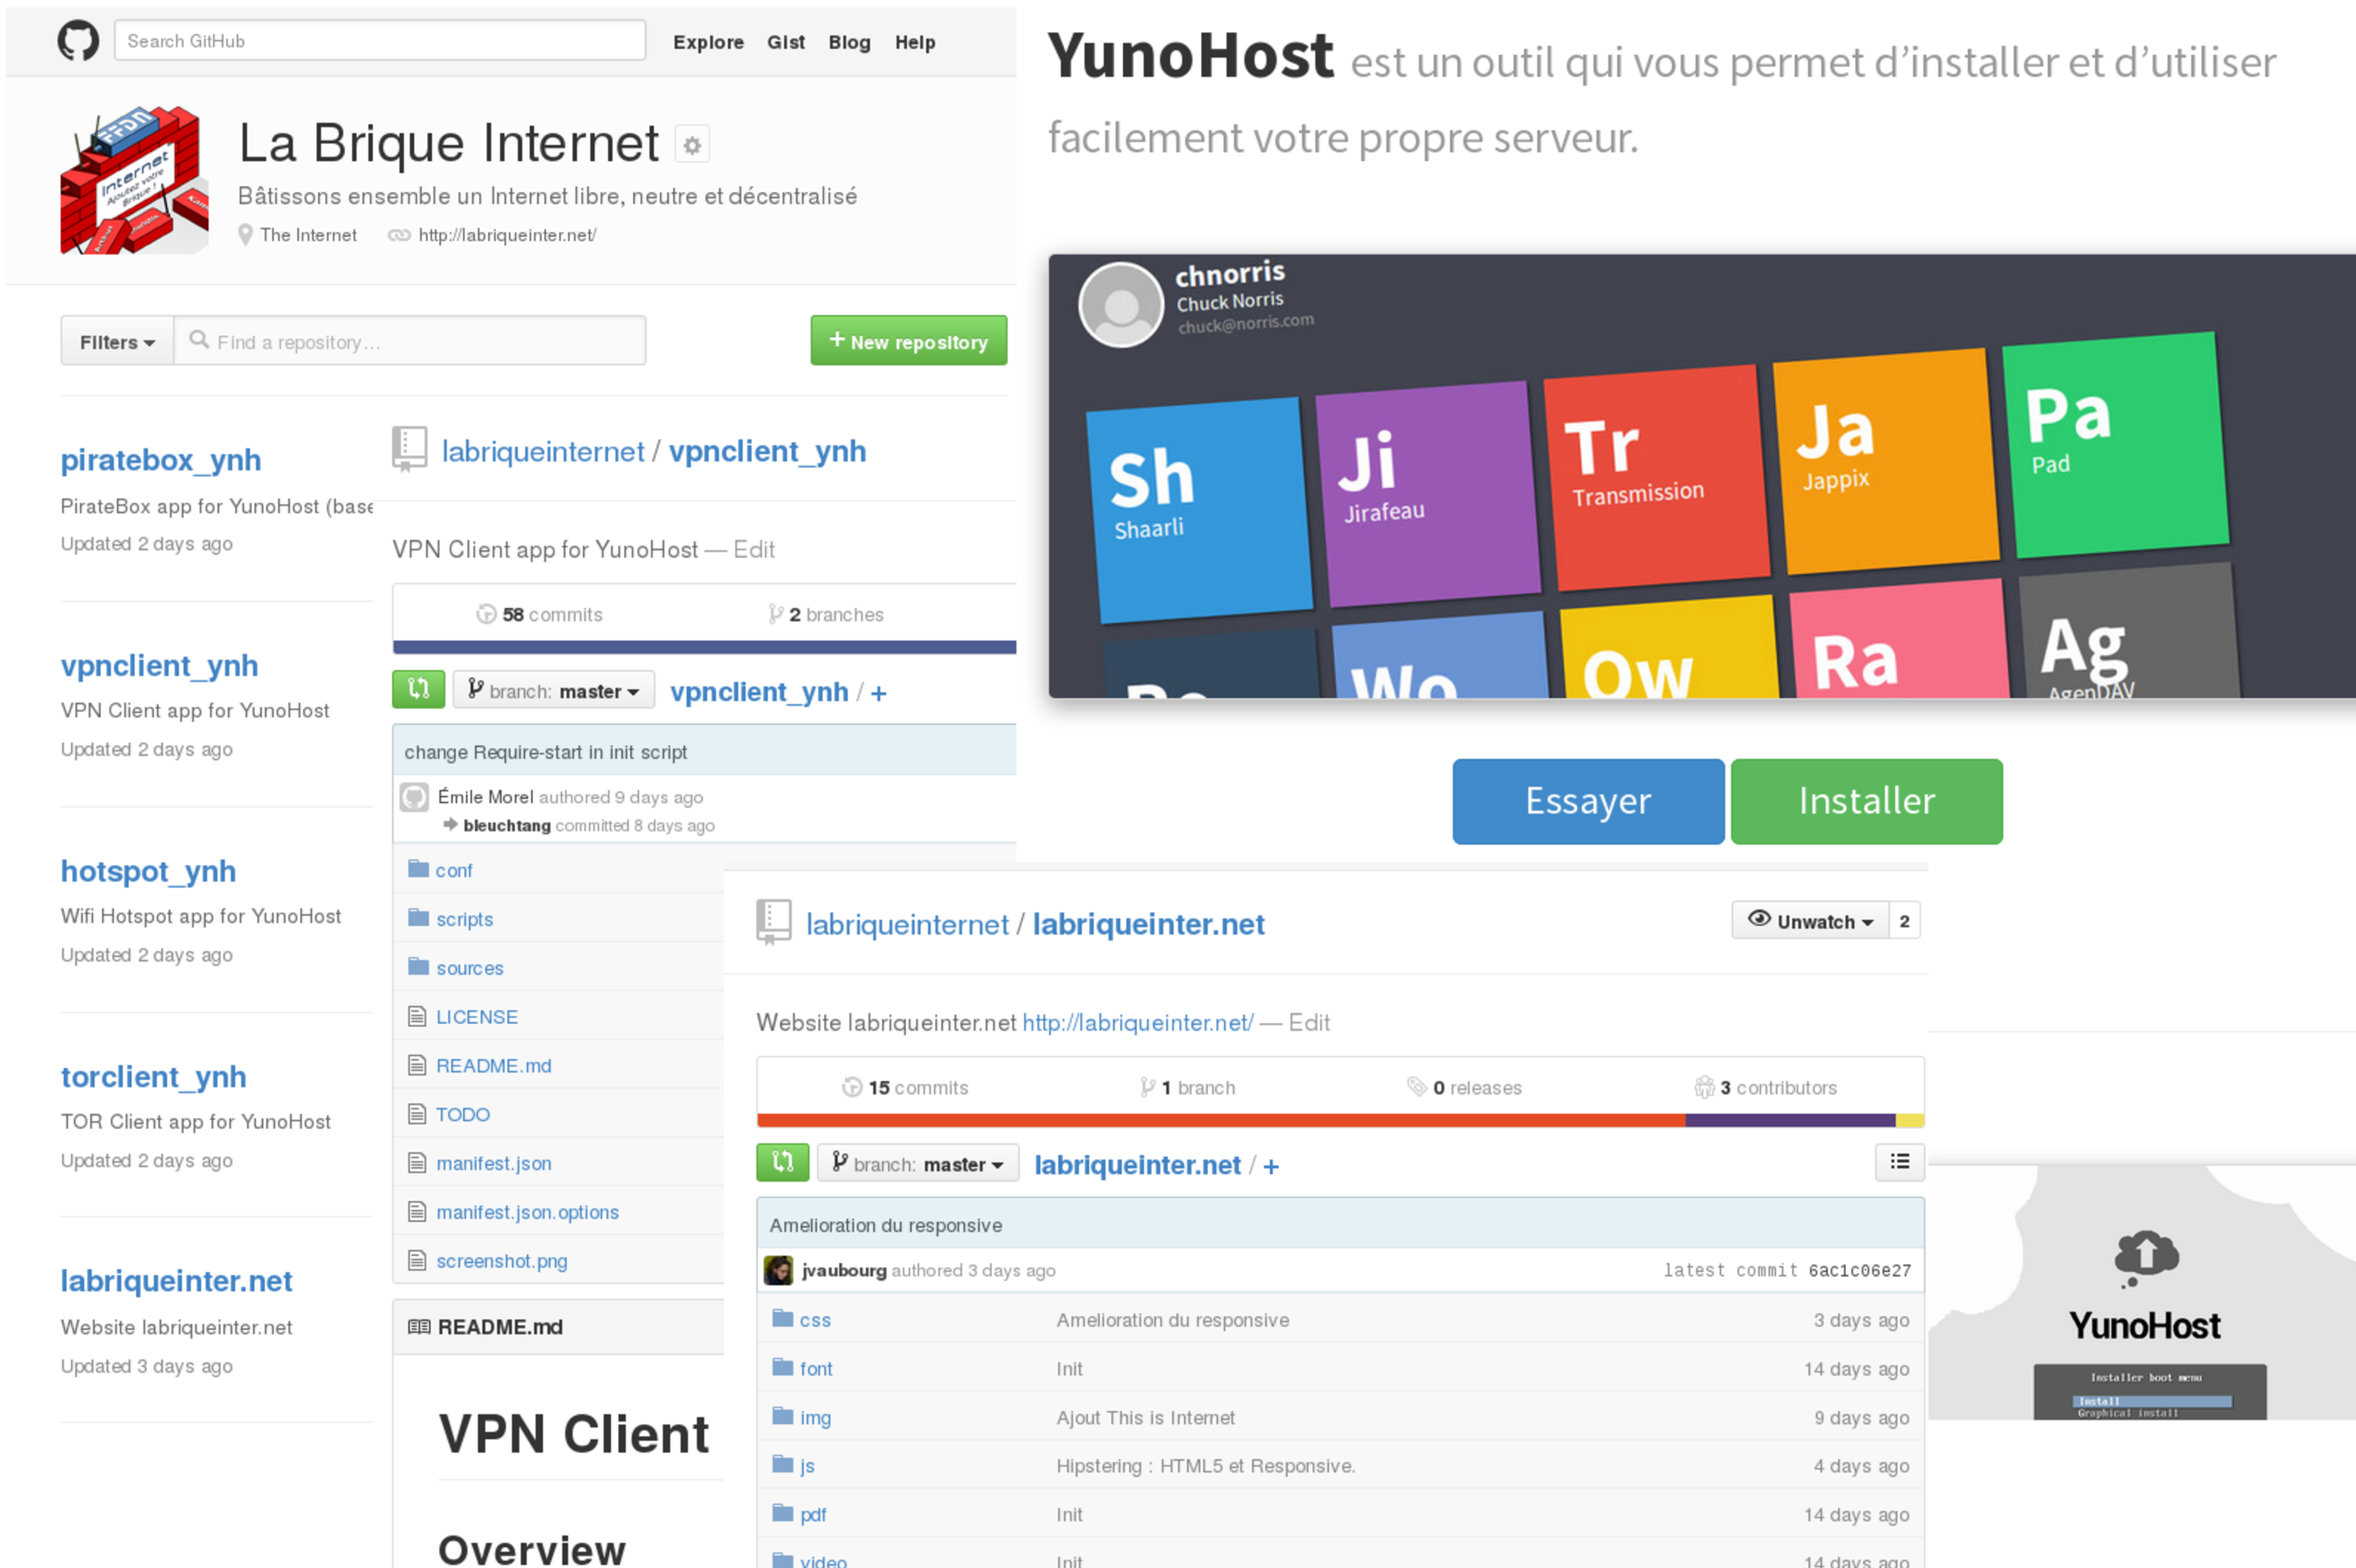
\includegraphics[width=10cm]{img2/25b-capture-github-contrib.pdf}
\vfill
\end{center}
\end{frame}

\begin{frame}[t]
\frametitle{\textcolor{titre}{Bilan}}
  \begin{center}
    La Brique Internet permet donc de :
    \vfill
    \begin{itemize}
      \item Facilement \textbf{nettoyer} son accès à Internet,
      \item et d'\textbf{autohéberger} des services et ses données sans être informaticien
    \end{itemize}
    \end{center}
    \vfill
    \pause
    Et c'est pas fini…
\end{frame}

\begin{frame}[t]
\frametitle{\textcolor{titre}{Et c'est pas fini…}}
\vfill
\begin{center}
\begin{itemize}
    \item Yunhost permet l'auto-hébergement facile (jabber, mail, …)
    \item Il suffit de se déplacer avec sa Brique pour
    \begin{itemize}
      \item avoir ses services, et ses données avec soi (vacances, déménagement)
      \item \textbf{pour conserver} son accès à Internet
      \item \textbf{partager} avec d'autres un accès à un Internet propre (événementiel)
    \end{itemize}
    \pause
  \item Nettoyer n'importe quel accès à Internet (exemple un accès 3 ou 4G)
  \item Avoir des \textbf{adresses ipv4 et ipv6 fixes}
\end{itemize}
\end{center}
\end{frame}



\begin{frame}[t]
\frametitle{\textcolor{titre}{Les applications de la Brique :}}
\vfill
\begin{center}
\begin{itemize}
    \item Connexion internet neutre par VPN
\end{itemize}
\end{center}
\end{frame}

\begin{frame}[t]
\frametitle{\textcolor{titre}{La brique VPN}}
\vfill
\begin{center}
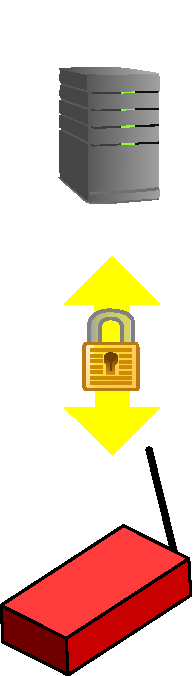
\includegraphics[scale=0.5]{img2/vpn.pdf}
\end{center}
\end{frame}

\begin{frame}[t]
\frametitle{\textcolor{titre}{Les applications de la Brique :}}
\vfill
\begin{center}
\begin{itemize}
    \item Connexion internet neutre par VPN
    \item Partage Box
\end{itemize}
\end{center}
\end{frame}

\begin{frame}[t]
\frametitle{\textcolor{titre}{La brique VPN}}
\vfill
\begin{center}
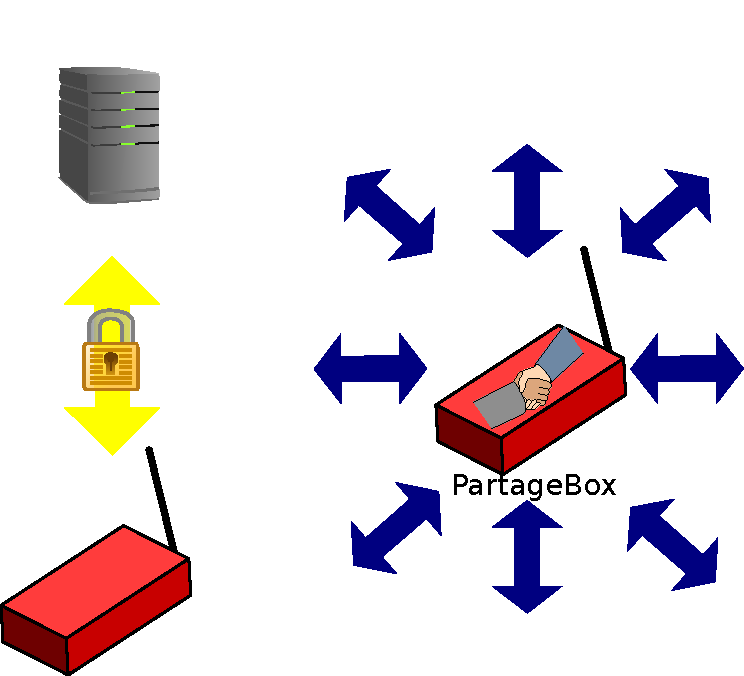
\includegraphics[scale=0.5]{img2/vpnpirate.pdf}
\end{center}
\end{frame}

\begin{frame}[t]
\frametitle{\textcolor{titre}{Les applications de la Brique :}}
\vfill
\begin{center}
\begin{itemize}
    \item Connexion internet neutre par VPN
    \item Partage Box
    \item Accès torifié
\end{itemize}
\end{center}
\end{frame}

\begin{frame}[t]
\frametitle{\textcolor{titre}{La brique VPN}}
\vfill
\begin{center}
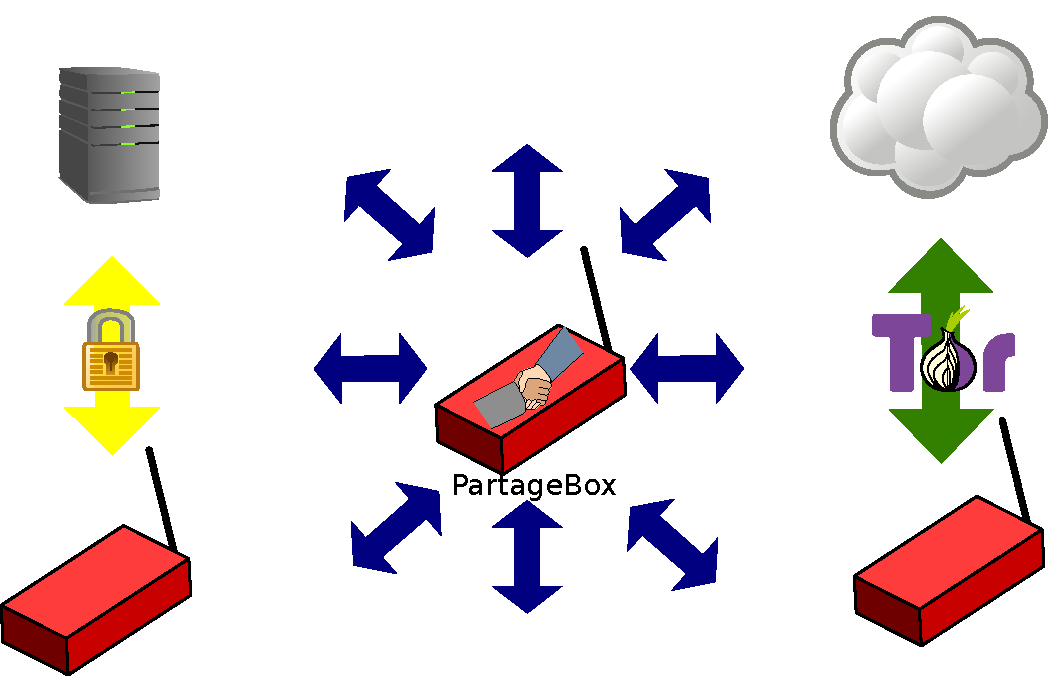
\includegraphics[scale=0.5]{img2/vpnpirator.pdf}
\end{center}
\end{frame}

\begin{frame}[t]
\frametitle{\textcolor{titre}{Les applications de la Brique :}}
\vfill
\begin{center}
\begin{itemize}
  \item Connexion internet neutre par VPN
  \item Partage Box
  \item Accès torifié
  \item Les 3 en même temps (multi SSID) \good
\end{itemize}
\end{center}
\end{frame}

\begin{frame}[t]
\frametitle{\textcolor{titre}{L'avenir}}
\vfill
\begin{center}
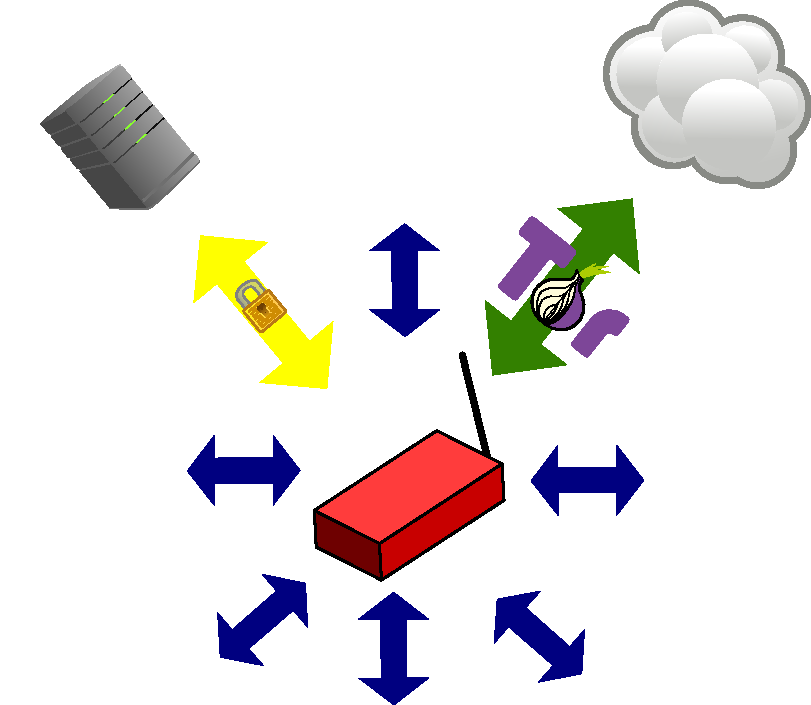
\includegraphics[scale=0.5]{img2/ultimate.pdf}
\end{center}
\end{frame}

\begin{frame}[t]
\frametitle{\textcolor{titre}{La Brique Internet, c'est donc}}
\vfill
\begin{itemize}
\item \textbf{s'émanciper} du pouvoir de son FAI \vfill
\item \textbf{reprendre le contrôle} sur ses services et ses données \vfill
\item \textbf{utiliser un Internet} propre sereinement \vfill
\item \textbf{jouer avec des logiciels libres}
\end{itemize}
\vfill
\end{frame}

\begin{frame}[t]
  \begin{center}
  %\vfill
  \vspace{.7cm}
  {\Huge \url{http://LaBriqueInter.Net}}
  \vspace{1cm}
  \begin{itemize}
    \item Discussions -- \url{https://listes.labriqueinter.net/}
    \item IRC -- \#labriqueinter.net sur irc.geeknode.org
    \item Images (en beta) -- \url{https://repo.labriqueinter.net/}
    \item Scripts de build -- \url{http://build.labriqueinter.net/}
    \item FAI Associatifs  -- \url{http://db.ffdn.org/}
  \end{itemize}
  \vspace{1cm}
  {\Huge discussions@listes.labriqueinter.net}
  \end{center}
\end{frame}

%\begin{frame}[t]
%\frametitle{\textcolor{titre}{J'ai une brique !}}
%\begin{center}
%  \vfill
%    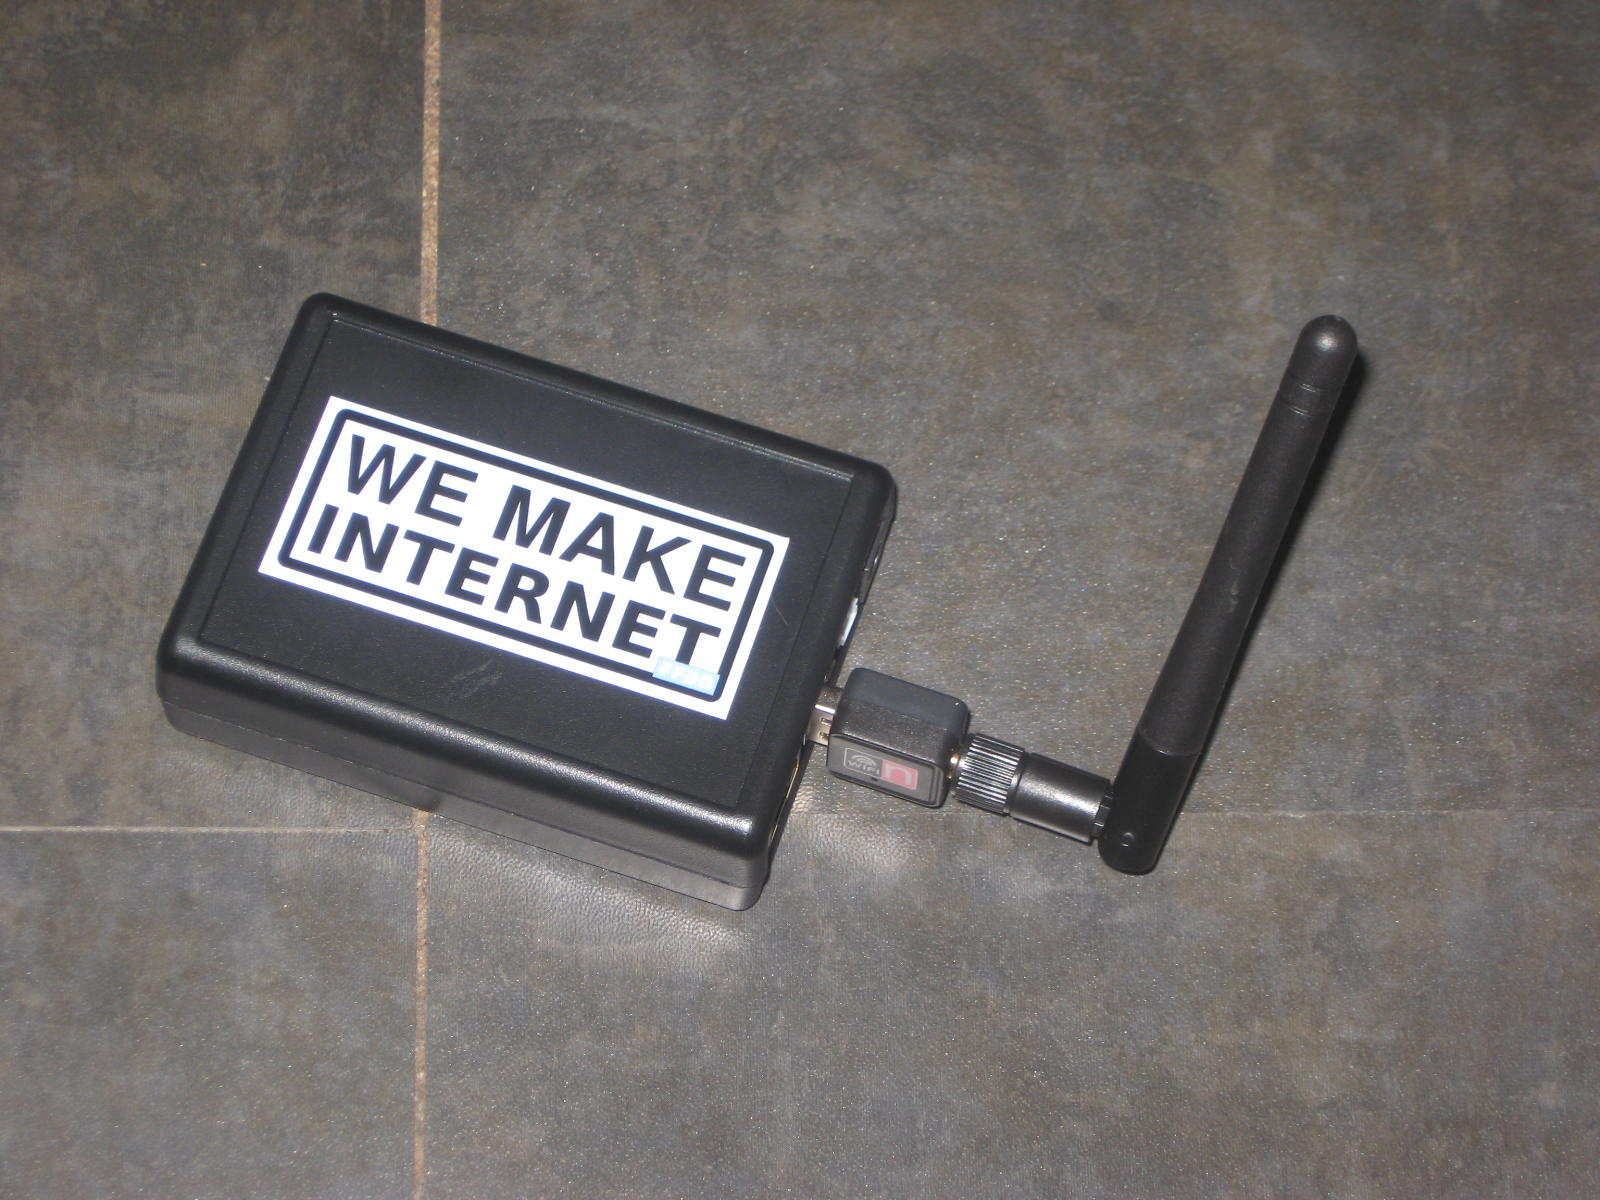
\includegraphics[width=.75\textwidth]{img2/04-photo-boitier.jpg}
%  \vfill
%\end{center}
%\end{frame}

\end{document}
